\documentclass[../main.tex]{subfiles}

\begin{document}


\section{Computation}

\subsection{Algorithms for Model Computation}

Given a set of physicians $\{(V_j, R_j(\cdot), \tau_j)\}_{j =1}^{J}$, punishment function $P(\cdot)$, distribution functions for patient parameters $F(\kappa)$ and $G(\gamma)$, and one search model parameter $z$, which is $\lambda$ in the Logit model, $\beta$ in the sequential model, we develop an algorithm to compute market equilibrium.

Equilibrium aggregates are computed on the basis of Monte-Carlo matrix calculus. Set $J$ as the number of physicians,\footnote{Or, as we'll later interpret it, as the number of bins, where each bin $j$ is a unique combination of $ (V_j, \tau_j, R_j(\cdot),P_j(\cdot))$.} $I$ as the size of the sample drawn randomly from $F(\kappa)$ and $G(\gamma)$. For both models we define a class which can output a matrix $S$ where each column is a patient's strategy vector $S_i$ following that model, when given as input the arrayed set of physicians' quality and visit cost $\{(V_j, \tau_j)\}_{i =1}^{J}$, an arrayed set of patients $(\{(\kappa_i,\gamma_i)\}_{i =1}^{I}$, the model parameter $z$ and a given vector of physician strategies $\{\bar{\kappa_j}\}_{j =1}^{J}$.

We input as ``patients'' our $I$ samples from $F(\kappa)$ and $G(\gamma)$, then a $J \times I$ matrix $U$ is computed, where each component $u_{ji}$ corresponds to the utility the sampled patient $i$ would get from a visit to physician $j$.\footnote{As we have defined our matrices $J \times I$ for ease of visualization, we will refer to matrix components as $x_{ji}$ in this section rather than $x_{ij}$ as we do elsewhere in the paper.} This step is the same for both classes.

What differs between both models is the computation of the matrix $S$ of patient strategis out of the utility matrix $U$:

\begin{itemize}[itemsep=4pt, topsep=0pt]
    \item \textbf{Implicit search model (Logit):} First, an `$\alpha$-matrix' is calculated over matrix $U,$ where each $\alpha_{ji}$ is $e^{\lambda u_{ji}}$ if $u_{ji} > 0$ and $0$ if not. Then, for each patient $i$, that is, for each column, each component $s_{ji}$ of the $S$ matrix takes on the values $s_{ji} = \alpha_{ji}/\sum_{k = 1}^{J} \alpha_{ki}$.

    \item \textbf{Explicit search model (Sequential):} Recall equation (NUMBER) characterizing patient thresholds. We first compute the $I$-dimensional vector of the sampled patients' respective $\bar{U_i}$. Define $U_i$ as the set $\{u_{ji}\}_{j=1}^{J}$ of utility patient $i$ recieves from a visit to each physician. In matrix terms $U_i$ would be the $i$th column of the $J \times I$ matrix $U$. The operation to compute each $\bar{U_i}$ is the following:
    \begin{equation*}
    \bar{U_i} \equiv \argmin_{x \, \in \, U_i}\; \left\|  \; x - \frac{\beta}{1-\beta}  \sum_{j=1}^{J} \left\{ \frac{\mathbbm{1}[ u_{ji} \geq x ] \cdot (u_{ji} - x)}{\mathbbm{1}[ u_{ji} \geq x ]} \right\} \right\|
    \label{eq:comp1}
    \end{equation*}
    where the norm $\| \cdot \|$ is defined in $\mathbb{R}$ as simply the absolute value $| \cdot |$. This is to say, for each sampled patient $i$ we evaluate $x$ for each $u_{ji}$ in $U_i$. In plain words, if patient $i$ where to say: ``I will only visit physicians which grant me at least as much utility as physician $j$'', the optimal choice of $j$ and its respective $u_{ji}$ would be the minimal in $U_i$ for the evaluation of the absolute value in the left-hand side of (\ref{eq:comp1}). This is computationally less intensive than seeking to compute the exact root of (NUMBER), which would be a redundant exercise, because there's a discrete number of physicians above that mark, and selecting instead to use ``the lowest $u_{ji}$ above the root of (NUMBER)'' as threshold instead of the root proper would result in the same vector of strategies $S_i$ for each patient.\footnote{Granted, this is not strictly true, as in our formulation a `$u_{ji}$' may be selected as threshold which is actually below the root proper in $\mathbb{R}$, but closer to it than the nearest one above it. The effect of this ``estimation noise'' on our overall results is negligible.}

    Once having computed our $I$-dimensional vector of patients' $\bar{U_i}$, we evaluate column-wise the binary operator $\mathbbm{1}\{u_{ji}\geq \bar{U_i}\}$ over matrix $U$, and the $J \times I$ matrix $S$ of patient strategies takes on the values $s_{ji} = \mathbbm{1}\{u_{ji}\geq \bar{U_i}\} / \sum_{k=1}^{J} \mathbbm{1}\{u_{ki}\geq \bar{U_i}\}$.
\end{itemize}

The $S$ matrix in both cases is computed in linear time, $\mathcal{O}(n)$ in big-O notation, where input size $n$ is the number of physicians $J$. Both consist of a series of ufunc or vectorized operations, where the inclusion of one more physician introduces a new row with $I$ elements on which operations are performed at each stage. The additional step of calculating the $\bar{U_i}$ vector makes the execution of the `explicit' search model relatively slower (see Figure \ref{fig:subfig1}).

\begin{figure}[H]
    \centering
    % First subfigure
    \begin{subfigure}[b]{0.45\linewidth}
        \centering
        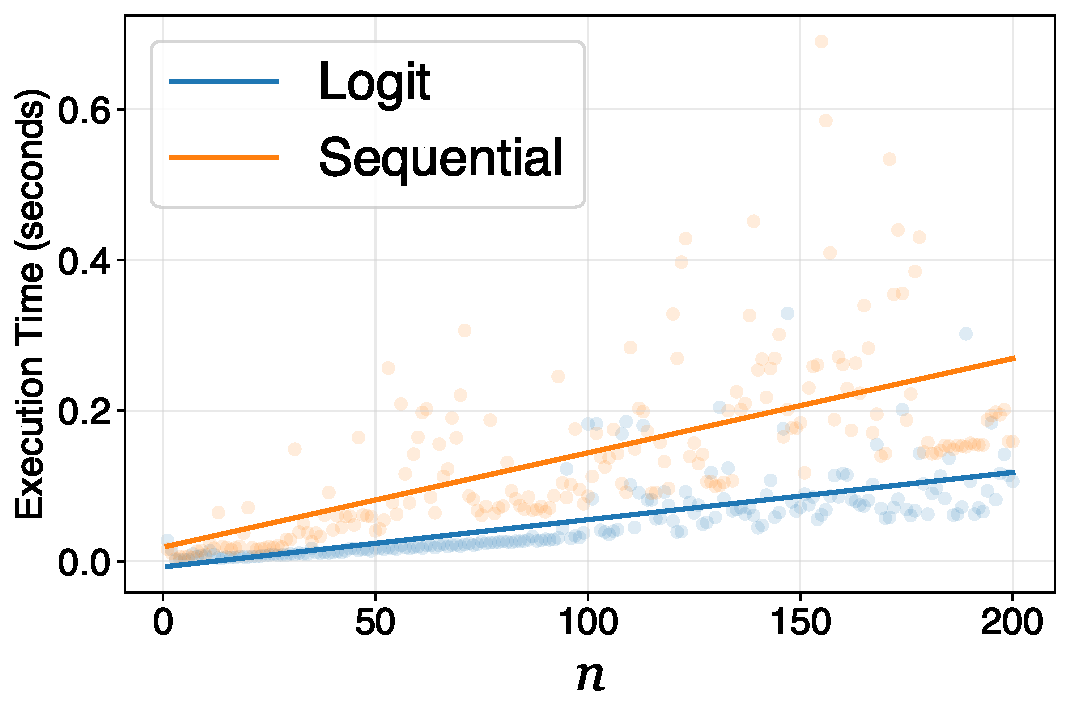
\includegraphics[width=\linewidth]{linear.pdf}
        \vspace{-0.6cm}
        \caption{Linear polynomial fit of execution time for $S$ matrix in both models}
        \label{fig:subfig1}
    \end{subfigure}
    \hspace{0.05\linewidth}  % Space between the subfigures
    % Second subfigure
    \begin{subfigure}[b]{0.45\linewidth}
        \centering
        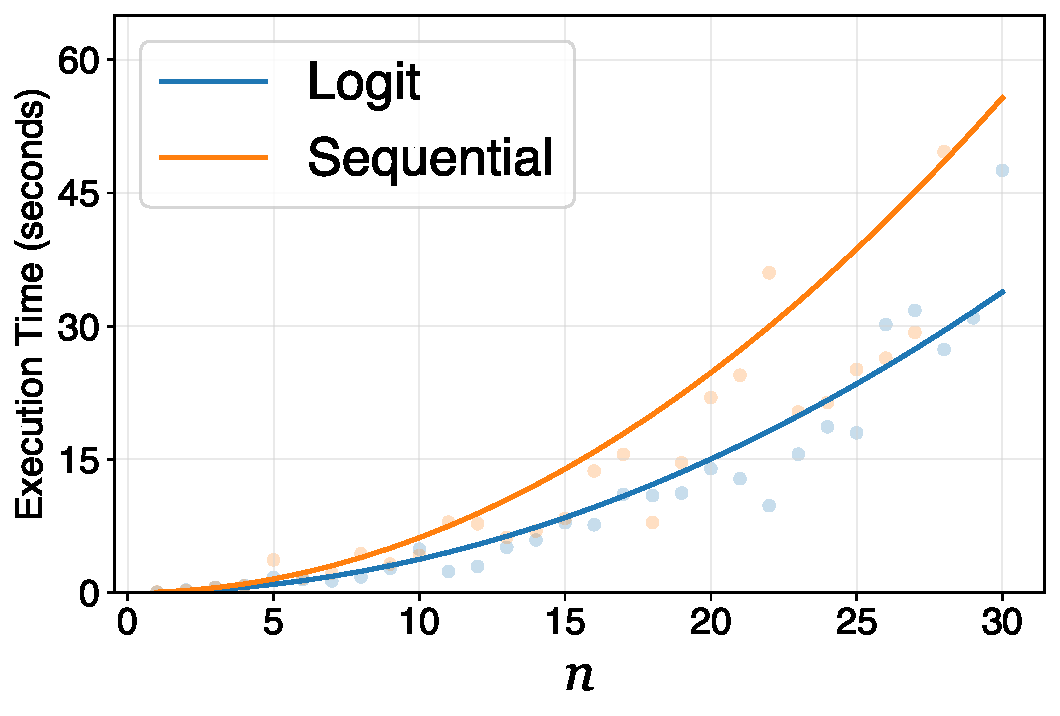
\includegraphics[width=\linewidth]{squared.pdf}
        \vspace{-0.6cm}
        \caption{Quadratic polynomial fit of execution time for $\bar{\kappa}^*$  vector in both models}
        \label{fig:subfig2}
    \end{subfigure}
    \caption{Execution time comparison \\ between the \textit{implicit} and \textit{explicit} search models}
    \label{fig:comp1}
\end{figure}

The steps following the computation of the $S$ matrix are the same for both models. The $J$-dimensional vector $Q$ of each physician's expected demand $Q_j$ is achieved through the row-wise summation of all patient's demand for $j$, i.e. performing $\sum_{i=1}^{I} s_{ji}$ for each $j$. The vector $X$ of each physician's expected sick leaves issued $X_j$ performs that same summation, conditional on the patients' $\kappa_i$ being above or at physician $j$'s chosen threshold $\bar{\kappa}_j$, that is, $\sum_{i=1}^{I}  \mathbbm{1}[ \kappa_{i} \geq \bar{\kappa}_j] \, s_{ji}$. Both sums are normalized to fit the actual number of patients in the physician-patient market.

For a given vector $\bar{\kappa}$, computing patient strategies, physician aggregates and then physicians' utility—defined as $\{R_j(Q_j) - P(X_j)\}$—entails a sequence of calculations done in linear time. However, the calculation of the \textit{equilibrium} vector $\bar{\kappa}^*$ is performed in quadratic time $\mathcal{O}(n^2)$, as it requires each of the aforementioned steps to be done some $x$ number of times \textit{per} physician, such that the inclusion of an additional physician increases the number of operations required \textit{per} physician as well as the amount of physicians whose $\bar{\kappa_j}$ needs to be computed. See Figure \ref{fig:subfig2}.

The algorithm to find the equilibrium $J$-vector $\bar{\kappa}^*$ of physician strategies is as follows:
\begin{enumerate}[label=\roman*, itemsep=0pt, topsep=0pt]
    \item Input an initial guess $\bar{\kappa}^0$ for physician thresholds.
    \item For each physician, we fix the the value of $\bar{\kappa}_{-j}$, the threshold values of the other $J-1$ physicians, and compute equilibrium aggregates and physician $j$'s utility for different choices of $\bar{\kappa}_{j}$ across a grid. In particular, $U_j(\bar{\kappa}_{j},\bar{\kappa}_{-j})$ is computed for each decimal step between 0 and $\bar{\kappa}_{\max}$, the maximum threshold physicians may choose.
    \item The choice of threshold $k_{j}$ which rendered $j$ the most utility in the previous step is selected, and a grid is set-up spanning the 19 centesimal values in $[k_j - 0.05, k_j + 0.05],$\footnote{If $k_j$ is 0 (or $\bar{\kappa}_{\max}$), only the 10 centesimal values above (below) and at $k_j$ are computed.} each value therein input as physician $j$'s threshold $\bar{\kappa}_{j}$ to compute $U_j$ again, and the value within the grid which maximizes utility is chosen as $\bar{\kappa}_j^1$.
    \item Having performed the previous step for all $J$ physicians, we input as a new guess the vector $\bar{\kappa}^1 = \{\bar{\kappa}_1^1,...,\bar{\kappa}_J^1\}$ to run steps ii and iii again. This defines an equilibrium-searching loop $\bar{\kappa}^{n} = \Phi(\bar{\kappa}^{n-1})$, and the loop is concluded when a fixed point is found, that is, the vector $\bar{\kappa}^*$ such that $\bar{\kappa}^{*} = \Phi(\bar{\kappa}^*)$.
    \item Optionally, having found a two decimals fixed point $\bar{\kappa}^*$, there's an algorithm in place to find an $x$-decimal fixed point $\bar{\kappa}^{*x}$. It starts by running a modified version of step iii on the two-decimal solution, setting up a grid of the 19 \textit{millesimal} values in $[\bar{\kappa}_j^{*} - 0.005, \bar{\kappa}_j^{*} + 0.005]$ for each physician $j$,\footnote{For $\bar{\kappa}_j^* = 0$ or $\bar{\kappa}_{\max}$ a similar logic to the footnote above follows.} selecting that which renders highest utility for each, and inputting this new vector as guess to run this step again, and so on until the fixed point $\bar{\kappa}^{* \scriptscriptstyle 3} = \Phi(\bar{\kappa}^{* \scriptscriptstyle 3})$ is found. 
    
    This goes on like this, calculating the $t$ decimals solution out of the $t-1$ decimals solution by setting up $10^{\text{-}(t-1)}$-sized grids for each physician in each iteration, until the specified amount of decimals wanted from the solution vector $\bar{\kappa}^{*x}$ is reached.
\end{enumerate}

On the one hand, having to perform several operations \textit{per} physician is quite computationally intensive and runs the cost of quadratic execution time. On the other hand, altough each iteration takes some time, for the right parameters the algorithm is quite efficient in the number of iterations needed for convergence, usually taking between 2 and 5. The option to find fixed points to \( n + 1 \) decimal places incurs progressively smaller execution time costs compared to \( n \) decimals, as the initial guess for \( n + 1 \) decimals becomes increasingly accurate. See Figure \ref{fig:decimals}.

\begin{figure}[H]
\centering
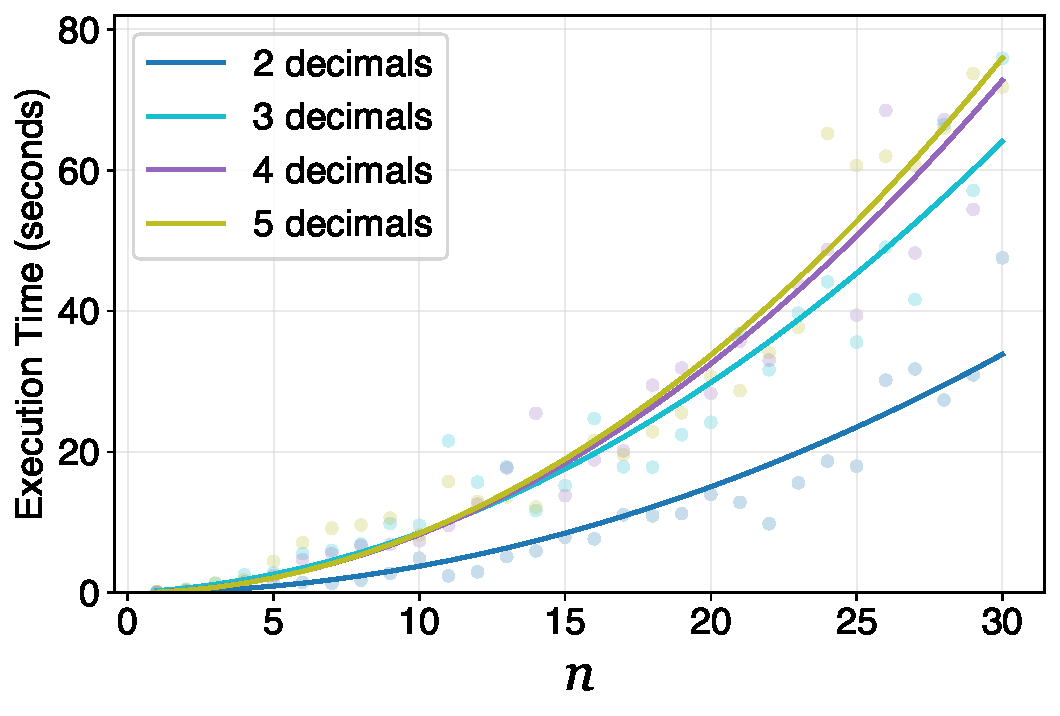
\includegraphics[width=0.55\linewidth]{decimals.pdf}
\vspace{-0.25cm}
\captionsetup{justification=centerlast}
\caption{Quadratic polynomial fit of execution time of $\bar{\kappa_j}^*$ \\ for different decimal approximations in Logit model}
\label{fig:decimals}
\end{figure}

Once the equilibrium vector $\bar{\kappa_j}^*$ is calculated, it may be used to compute the equilibrium aggregates $Q_j$ and $X_j$ for all physicians, as well as physician utility.

\subsection{Illustrative Examples}

\begin{figure}[H]
    \centering
    % First subfigure
    \begin{subfigure}[b]{0.46\linewidth}
        \centering
        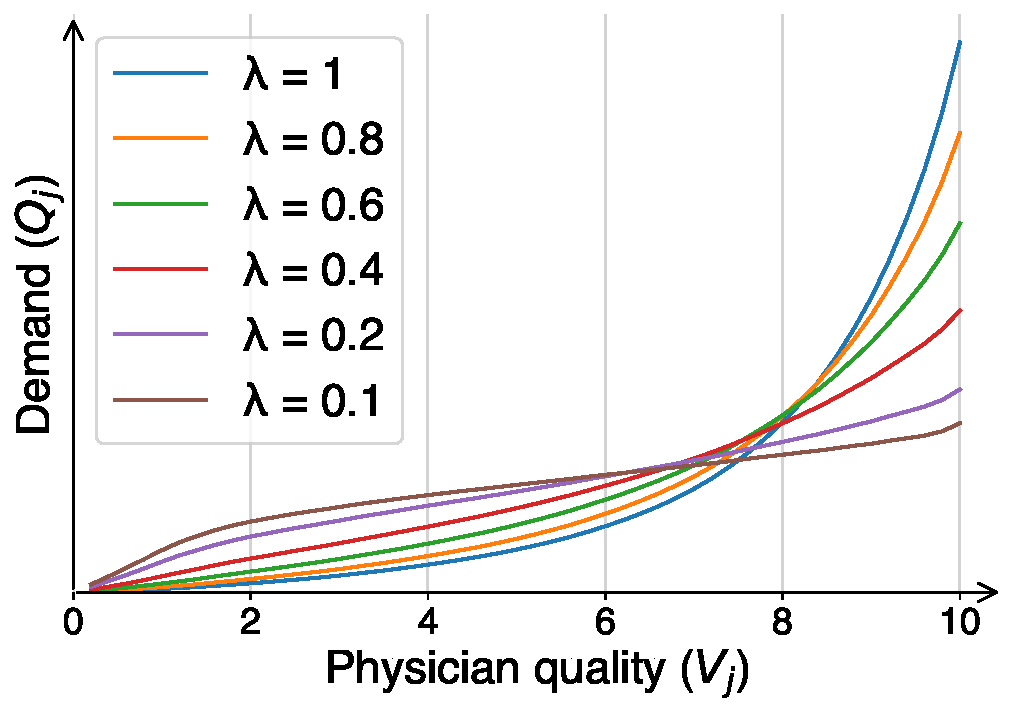
\includegraphics[width=\linewidth]{Q_zero.pdf}
        \vspace{-0.6cm}
        \caption{Patient demand $Q_j$ \\ by physician quality, $\bar{\kappa} = \vec{0}$}
        \label{fig:LogitQ0}
    \end{subfigure}
    \hspace{0.05\linewidth}  % Space between the subfigures
    % Second subfigure
    \begin{subfigure}[b]{0.46\linewidth}
        \centering
        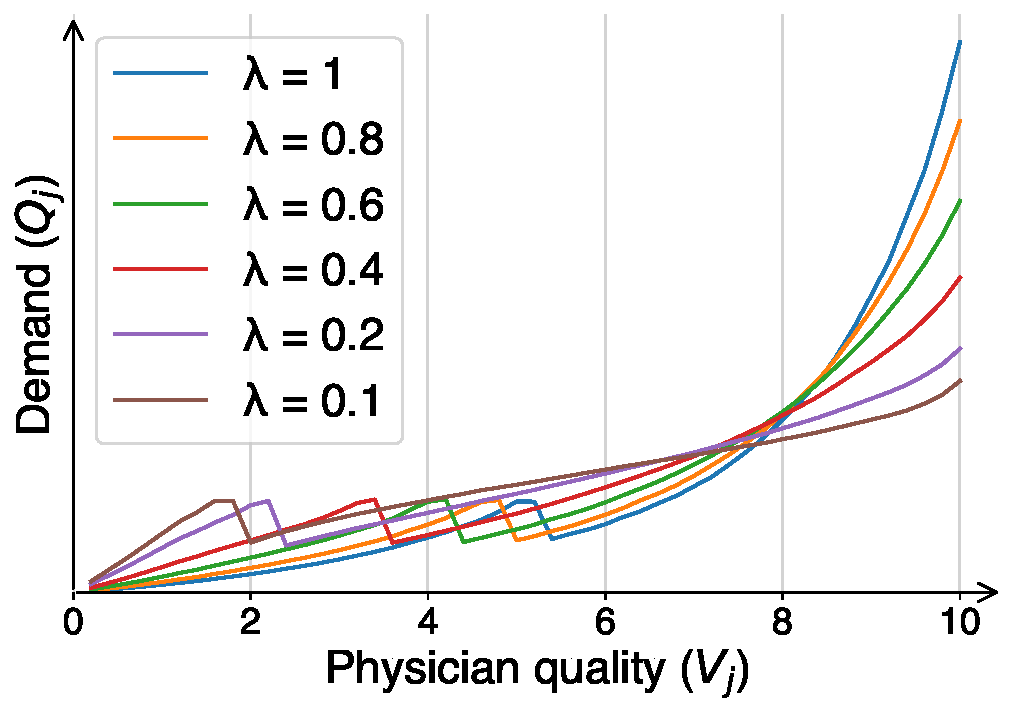
\includegraphics[width=\linewidth]{Q_eq.pdf}
        \vspace{-0.6cm}
        \caption{Patient demand $Q_j$ \\ by physician quality, equilibrium $\bar{\kappa}^*$}
        \label{fig:LogitQeq}
    \end{subfigure}

    \vspace{0.5cm}

    \begin{subfigure}[b]{0.46\linewidth}
        \centering
        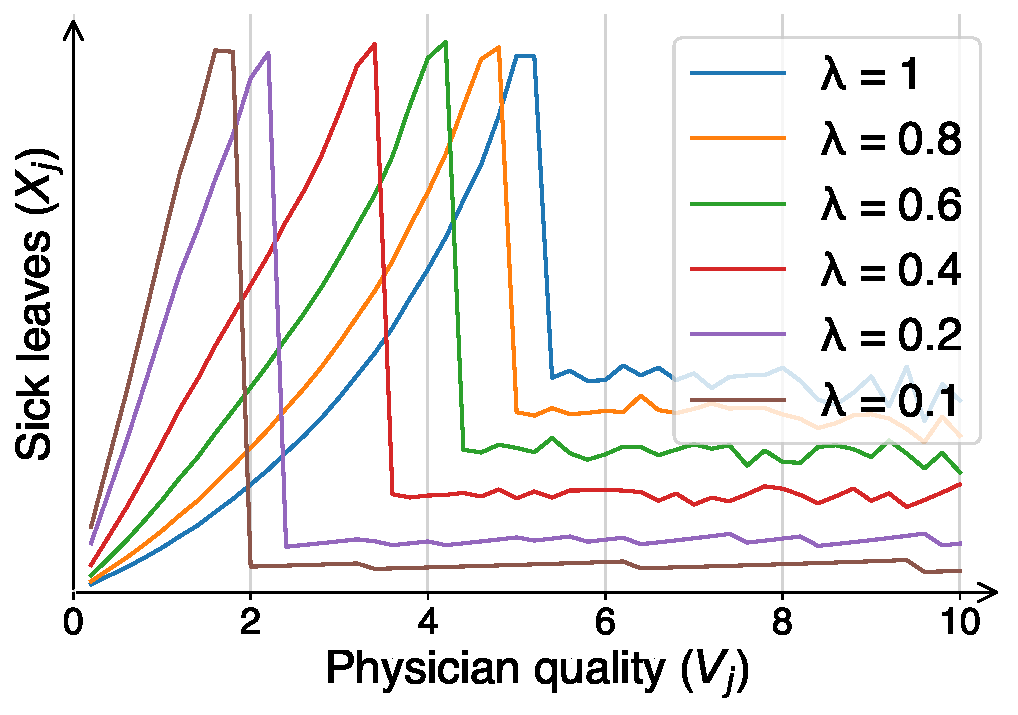
\includegraphics[width=\linewidth]{X.pdf}
        \vspace{-0.6cm}
        \caption{Sick leaves issued $X_j$ \\ by physician quality, equilibrium $\bar{\kappa}^*$}
        \label{fig:LogitX}
    \end{subfigure}
    \hspace{0.05\linewidth}  % Space between the subfigures
    % Second subfigure
    \begin{subfigure}[b]{0.46\linewidth}
        \centering
        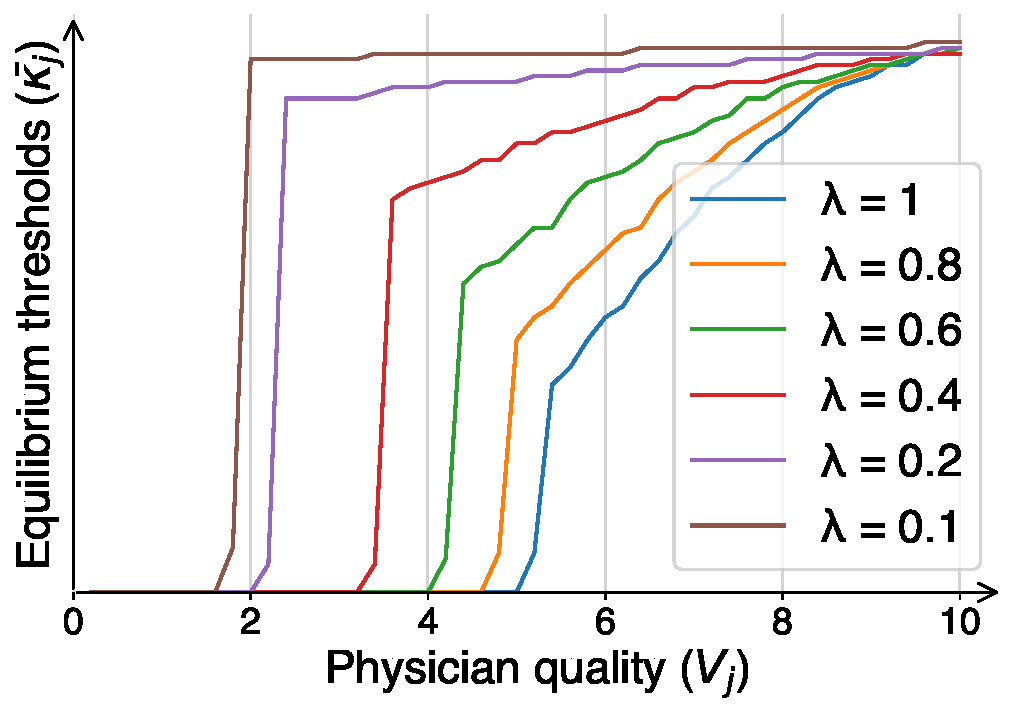
\includegraphics[width=\linewidth]{ks.pdf}
        \vspace{-0.6cm}
        \caption{Equilibrium $\bar{\kappa_j}^*$ by physician quality \\ \text{}}
        \label{fig:Logitk}
    \end{subfigure}

    \caption{Physician aggregates and strategies for different values of $\lambda$ \\ in the \textit{implicit} search model}
    \label{fig:Logit}
\end{figure}

\newpage

\begin{figure}[H]
    \centering
    % First subfigure
    \begin{subfigure}[b]{0.46\linewidth}
        \centering
        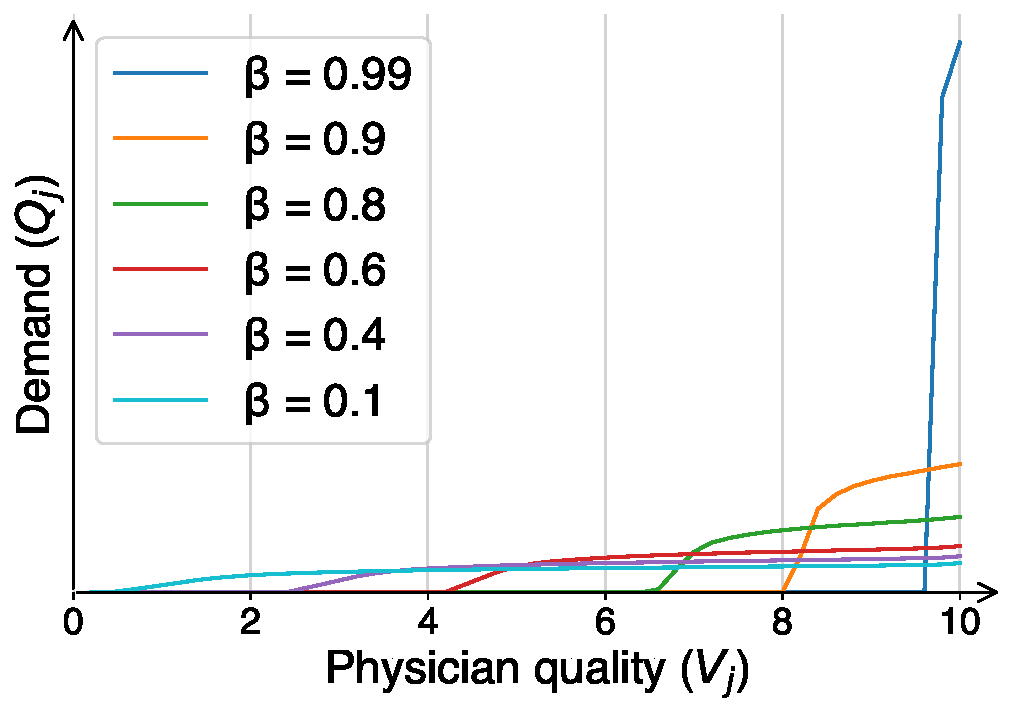
\includegraphics[width=\linewidth]{schnell_Q_0.pdf}
        \vspace{-0.6cm}
        \caption{Patient demand $Q_j$ \\ by physician quality, $\bar{\kappa} = \vec{0}$}
        \label{fig:SchnellQ0}
    \end{subfigure}
    \hspace{0.05\linewidth}  % Space between the subfigures
    % Second subfigure
    \begin{subfigure}[b]{0.46\linewidth}
        \centering
        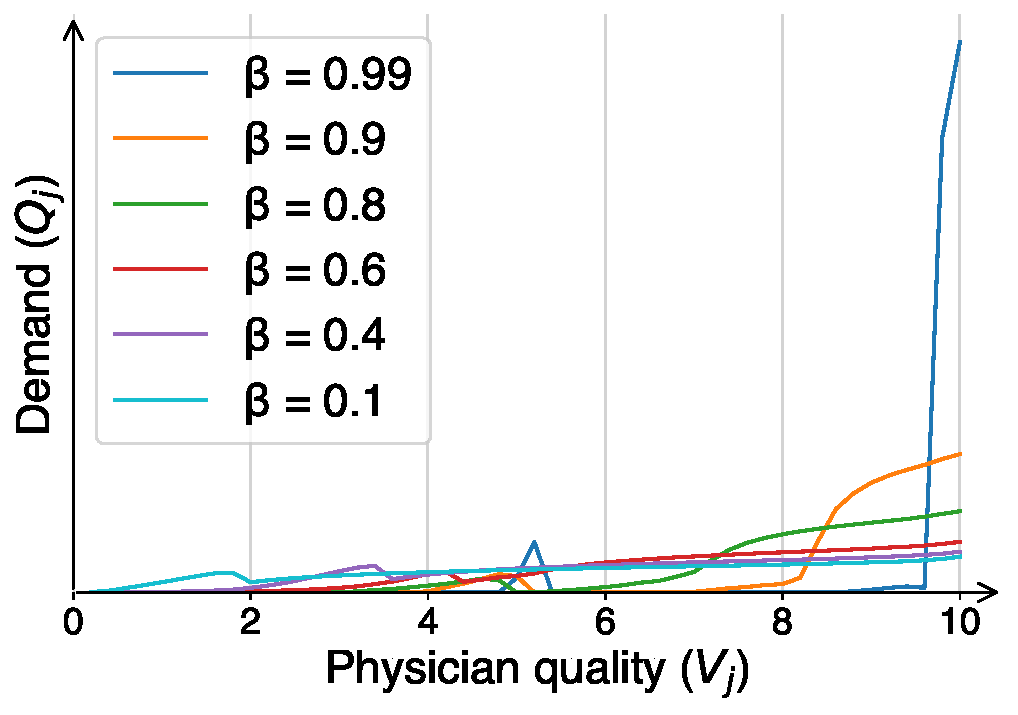
\includegraphics[width=\linewidth]{schnell_Q_eq.pdf}
        \vspace{-0.6cm}
        \caption{Patient demand $Q_j$ \\ by physician quality, equilibrium $\bar{\kappa}^*$}
        \label{fig:SchnellQeq}
    \end{subfigure}

    \vspace{0.5cm}

    \begin{subfigure}[b]{0.46\linewidth}
        \centering
        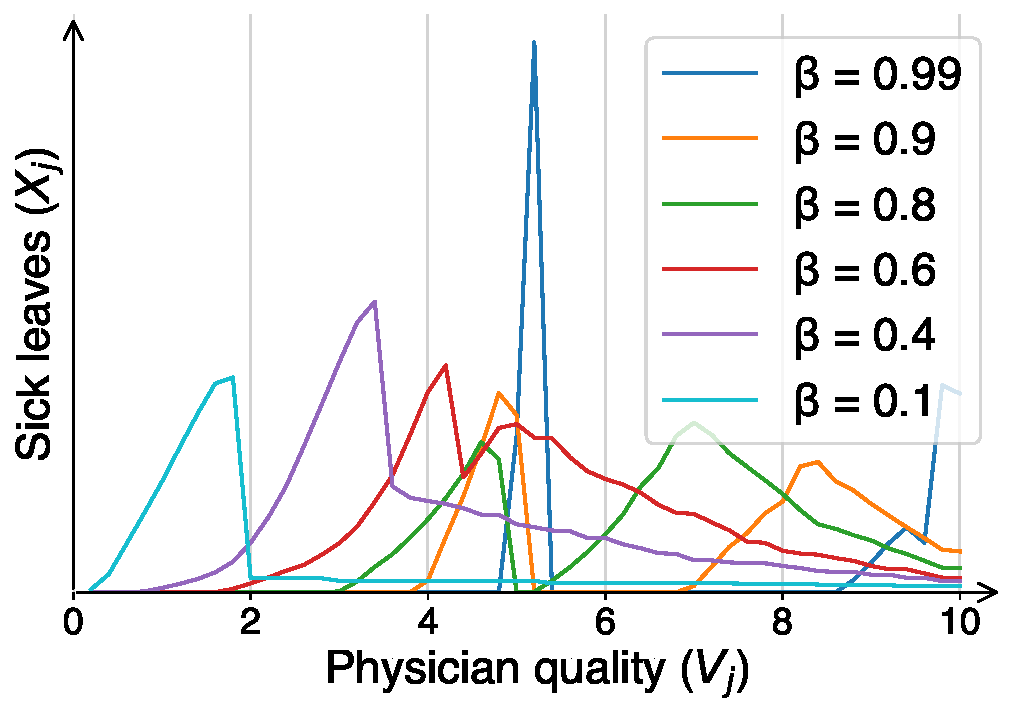
\includegraphics[width=\linewidth]{schnell_X.pdf}
        \vspace{-0.6cm}
        \caption{Sick leaves issued $X_j$ \\ by physician quality, equilibrium $\bar{\kappa}^*$}
        \label{fig:SchnellX}
    \end{subfigure}
    \hspace{0.05\linewidth}  % Space between the subfigures
    % Second subfigure
    \begin{subfigure}[b]{0.46\linewidth}
        \centering
        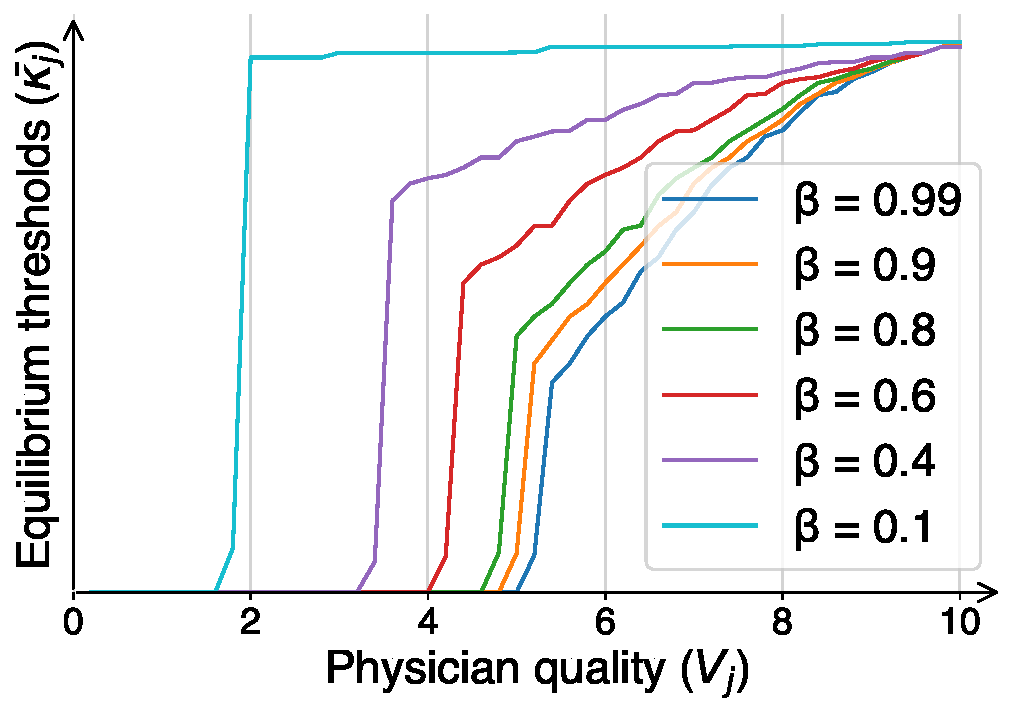
\includegraphics[width=\linewidth]{schnell_ks.pdf}
        \vspace{-0.6cm}
        \caption{Equilibrium $\bar{\kappa_j}^*$ by physician quality \\ \text{}}
        \label{fig:Schnellk}
    \end{subfigure}

    \vspace{0.5cm}

    \begin{subfigure}[b]{0.46\linewidth}
        \centering
        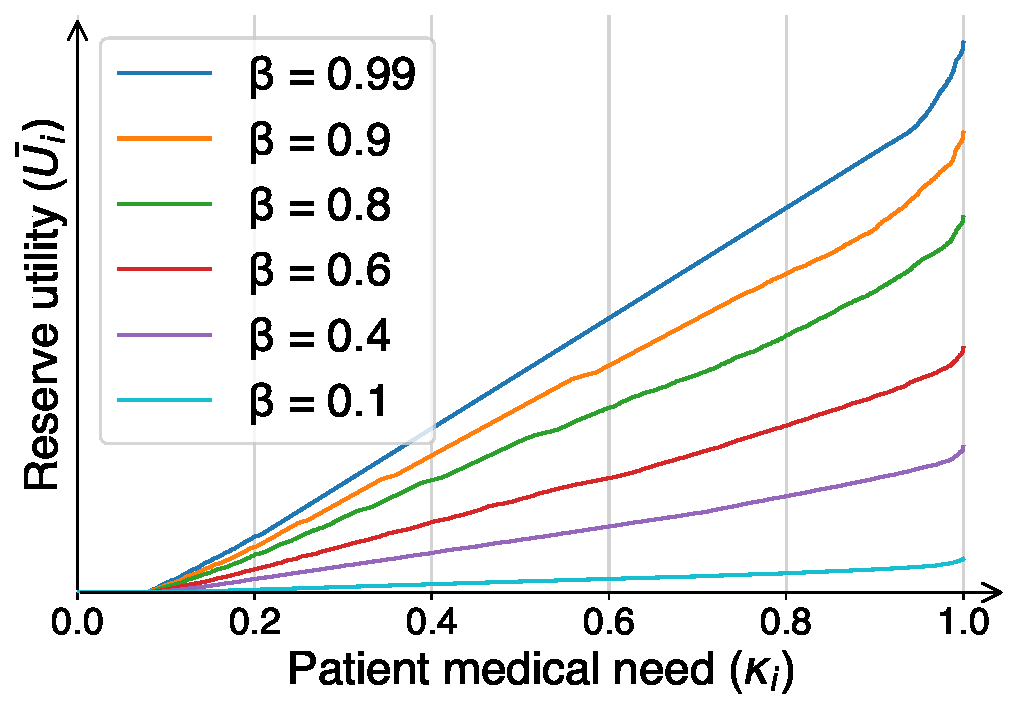
\includegraphics[width=\linewidth]{patient_uroot.pdf}
        \vspace{-0.6cm}
        \caption{Patient reserve utility $\bar{U_i}$ \\ by medical necessity ($\kappa_i$), equilibrium $\bar{\kappa}^*$}
        \label{fig:SchnellX}
    \end{subfigure}
    \hspace{0.05\linewidth} 

    \caption{Physician aggregates and strategies for different values of $\beta$ \\ in the \textit{explicit} search model}
    \label{fig:Schnell}
\end{figure}

\end{document}